\documentclass[a4paper, 11pt]{article}
\usepackage[utf8]{inputenc} 
\usepackage[T1]{fontenc}
\usepackage[catalan]{babel}
\usepackage{amsmath, amssymb, amsthm}
\usepackage[margin=1in]{geometry}
\usepackage{enumerate}
\usepackage{array}
\usepackage{graphicx}
\usepackage{wrapfig}
\usepackage{ragged2e} 
\usepackage{subfig}
\usepackage{caption}
\usepackage{subcaption}
\usepackage[dvipsnames]{xcolor}
%\usepackage[table]{xcolor}
\usepackage{float}
\usepackage{chngcntr}
\usepackage{ragged2e}
\usepackage{multirow}
\usepackage{vmargin}
\usepackage{hyperref}
\usepackage{url}
\usepackage{fancyhdr}
\usepackage{bigints}
\usepackage{listings}
\usepackage{xcolor,colortbl}
\usepackage{longtable}
\usepackage{multimedia}



\definecolor{bluebell}{rgb}{0.64, 0.64, 0.82}
\definecolor{atomictangerine}{rgb}{1.0, 0.6, 0.4}
\definecolor{applegreen}{rgb}{0.55, 0.71, 0.0}
\definecolor{frenchblue}{rgb}{0.0, 0.45, 0.73}
\definecolor{darkpastelgreen}{rgb}{0.01, 0.75, 0.24}
\definecolor{darkpastelblue}{rgb}{0.47, 0.62, 0.8}
\definecolor{navy}{rgb}{0,0,128}
\definecolor{codegreen}{rgb}{0,0.6,0}
\definecolor{codegray}{rgb}{0.5,0.5,0.5}
\definecolor{codepurple}{rgb}{0.58,0,0.82}
\definecolor{backcolour}{rgb}{0.95,0.95,0.92}
\definecolor{amaranth}{rgb}{0.9, 0.17, 0.31}
\definecolor{GRAY}{rgb}{0.75, 0.75, 0.75}
\definecolor{deepfuchsia}{rgb}{0.76, 0.33, 0.76}
\definecolor{deepmagenta}{rgb}{0.8, 0.0, 0.8}
\definecolor{funcblue}{rgb}{0.36, 0.57, 0.9}
\definecolor{navy}{rgb}{0,0,128}
\definecolor{codegreen}{rgb}{0,0.6,0}
\definecolor{codegray}{rgb}{0.5,0.5,0.5}
\definecolor{codepurple}{rgb}{0.58,0,0.82}
\definecolor{backcolour}{rgb}{0.95,0.95,0.92}
\definecolor{amaranth}{rgb}{0.9, 0.17, 0.31}
\definecolor{GRAY}{rgb}{0.75, 0.75, 0.75}
\definecolor{deepfuchsia}{rgb}{0.76, 0.33, 0.76}
\definecolor{deepmagenta}{rgb}{0.8, 0.0, 0.8}
\definecolor{funcblue}{rgb}{0.36, 0.57, 0.9}

\lstdefinelanguage{GERONA}{
    classoffset = 1,
    morekeywords = {for, if, else, while, ifelse, in, return},
    keywordstyle = \color{atomictangerine},
    classoffset = 2,
    alsoletter=\#,
    morekeywords = {function, pmax, append, floor, length, plot, lines, rep, sum, matrix, solve},
    keywordstyle = \color{bluebell},
    classoffset = 0,
    sensitive = true,
    morecomment = [l]{#},
    commentstyle = \color{applegreen},
    morestring = [b]",
    morestring = [b]',
    stringstyle = \color{applegreen}
}


\begin{document}
\begin{titlepage}
    \centering
    {\bfseries\LARGE \hspace{1.9em} Universitat Autònoma de Barcelona\newline Facultat de Ciències\par}
    \vspace{2cm}
    {\hspace{-1em}
\includegraphics[width=0.6\textwidth]{MatCAD3.jpg}\par}
    \vspace{1cm}
    {\scshape\Huge Pràctica 2\par} 
    \vspace{1cm}
    {\Large \itshape Autors: \par}
    \vspace{0.5cm}
    {\Large \hspace{-1.5 em}Gerard Lahuerta \& Ona Sánchez \par}
    \vspace{0.5cm}
    {\Large 1601350 --- 1601181 \par}
    \vspace{1cm}
    {\Large 20 de Gener del 2023\par}
\end{titlepage}

\justifying

\newpage
{
\small
\setcounter{page}{2}
\pagestyle{plain}
\tableofcontents
\cleardoublepage
\addcontentsline{}{chapter}{}
}
\newpage
\section{Resolució apartat 1}\label{apartat1}
Per tal de trobar la solució al sistema d'$EDP$ plantejat, s'ha utilitzat un codi d'$R$ que es pot consultar a l'apartat \textcolor{blue}{\ref{annex}}.\\\\
Representem ara la trajectòria que descriu el punt mig de la corda en funció del temps, utilitzant la condició inicial $u_{0}(x) = x \cdot (1-x)$.\\\\
Els paràmetres de la simulació són:
\begin{table}[h]
    \centering
    \begin{tabular}{ccccccc}
        $v_{0} = 0$; & $c(x) = 1$; & $M = 200$; & $g(t) = 0$; & $\Delta x = \frac{1}{M-1}$; & $\Delta t = \Delta x$; & $t_f = 10$\\
    \end{tabular}
\end{table}
\\
S'obtenen els següents gràfics per diferents valors de $\gamma$:
\vspace{-1.8em}
\begin{figure}[h]
\captionsetup[subfigure]{labelformat=empty}
\centering
  \subfloat[Valor de $u(0.5,t)$ amb $\gamma = 0.2$]{
    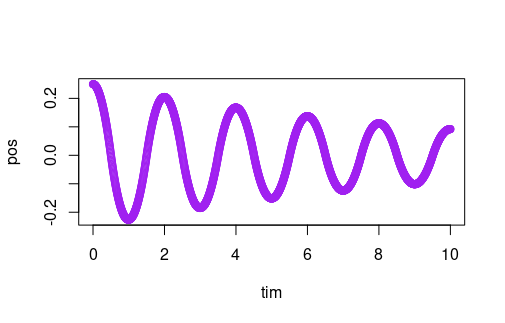
\includegraphics[width=0.5\textwidth]{imageeeee1.png}}
  \subfloat[Valor de $u(0.5,t)$ amb $\gamma = 0$]{
    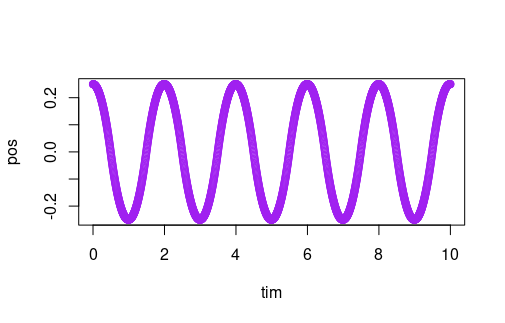
\includegraphics[width=0.5\textwidth]{imageeee2.png}}
\end{figure}\\
On s'observa que el període d'oscil·lació és aproximadament 2 per ambdós casos.\\\\
Destacar també que la modificació del paràmetre $\gamma$ genera canvis al gràfic ja que simula el fregament de la corda, de manera que al gràfic de la dreta, de forma ideal, $\gamma$ és igual a 0 i per tant la trajectòria no varia, mentre que al gràfic de l'esquerra la posició tendeix a 0.\\\\
Repetint la simulació usant $u_{0}(x) = 5x^{2} \cdot (1-x)^{2}$ s'obtenen els següents resultats:
\vspace{-1.8em}
\begin{figure}[h]
\captionsetup[subfigure]{labelformat=empty}
\centering
  \subfloat[Valor de $u(0.5,t)$ amb $\gamma = 0.2$]{
    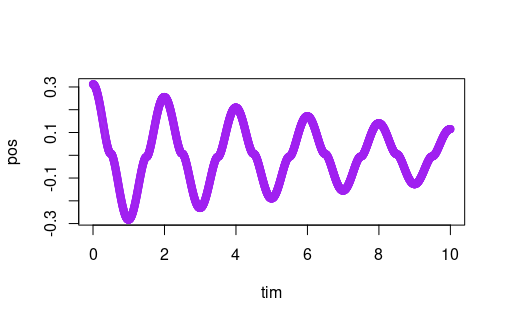
\includegraphics[width=0.5\textwidth]{imageeeee4.png}}
  \subfloat[Valor de $u(0.5,t)$ amb $\gamma = 0$]{
    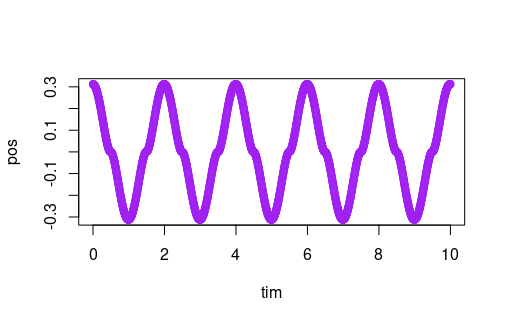
\includegraphics[width=0.5\textwidth]{imageeee3.png}}
\end{figure}\\
On s'observa que el període d'oscil·lació (T=2) és independent de la condició inicial $u_{0}$, tot i que la trajectòria del punt mig si que varia depenent de la condició inicial de la corda.

\newpage
\section{Resolució apartat 2}
Abans de crear una funció que aproximi de manera numèrica l'energia de la corda en el temps; reescribim la funció aproximant les derivades per diferencies finites i l'integral com a sumatori.\\
\begin{equation*}
    E(t) = \frac{T}{2}\int_0^1 \left[ \frac{1}{c(x)} \left( \partial_t u(x,t) \right)^2 + \left( \partial_x u(x,t) \right)^2 \right] dx
    \approx
\end{equation*}\begin{equation*}
    \approx \frac{T}{2}\sum_{i = 2}^{M-2} \left[ \frac{1}{c(x)} \left( \frac{U_i - U'_i}{\Delta t} \right)^2 + \left( \frac{U_i - U_{i-1}}{\Delta x} \right)^2 \right] \Delta x
\end{equation*}
\\
On $\Delta x$ i $\Delta t$ son els increments de temps, $\Delta x = \frac{x_f- x_i}{n}$ amb $n$ nombre d'intervals i $x_f$ i $x_i$ els extrems final i inicial de la corda respectivament; $U$ és un vector que aproxima la funció $u(x,t)$ on cada element és un interval de la corda i $U'$ és un vector que aproxima la funció $u(x,t)$ peró en un interval de temps anterior (son els valors que abans tenia el vector $U$).\\\\
Amb aquesta aproximació podem ara crear la funció que aproximi l'equació de l'energia de la corda:\\
\begin{lstlisting}[language = GERONA]
Energy = function(Up, U){
  ret = c()
  for ( i in 2:(length(U)) ){
    res = ( ((U[i]-Up[i])/dt)**2+((U[i]-U[i-1])/dx)**2 )
    ret = c(ret, res)
  }
  ret = 0.5*sum(ret)* dx
  return(ret)
}
\end{lstlisting}
\vspace{1em}
Aquesta funció calcula l'energia en un temps concret, pel que la introduïm en el bucle que calcula la posició dels intervals de la corda per així obtenir un gràfic amb la corva que segueix l'energia de la corda, tal i com s'observa al codi que es pot consultar a \textcolor{blue}{\ref{annex}}.
\newpage
\section{Resolució apartat 3}
Grafiquem ara l'energia de la corda en funció del temps per als paràmetres definits a \textcolor{blue}{\ref{apartat1}} i amb valors de $\gamma \in \{0, 0.2\}$ i $M \in \{200, 500\}$.
\vspace{-2em}
\begin{figure}[h]
\captionsetup[subfigure]{labelformat=empty}
\centering
  \subfloat[$\gamma = 0.2$]{
    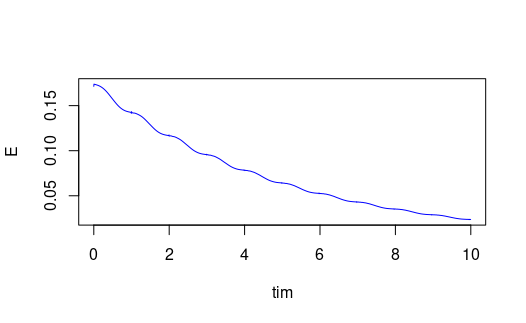
\includegraphics[width=0.5\textwidth]{gam02m200.png}}
  \subfloat[$\gamma = 0$]{
    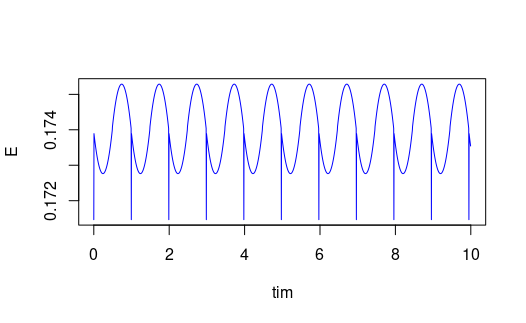
\includegraphics[width=0.5\textwidth]{gam0m200.png}}
   \caption{Gràfics amb valor $M = 200$}
\end{figure}
\vspace{-2em}
\begin{figure}[h]
\captionsetup[subfigure]{labelformat=empty}
\centering
  \subfloat[$\gamma = 0.2$]{
    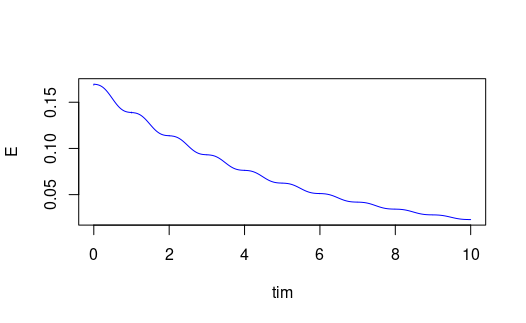
\includegraphics[width=0.5\textwidth]{gam02m500.png}}
  \subfloat[$\gamma = 0$]{
    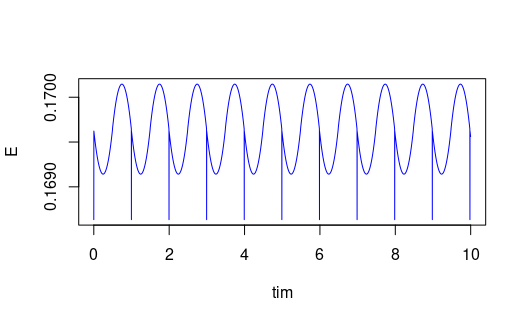
\includegraphics[width=0.5\textwidth]{gam0m500.png}}
   \caption{Gràfics amb valor $M = 500$}
\end{figure}
\\\\
S'observa com la tendència quan la $\gamma$ és major a 0 és a decrementar l'energia, per contra a quan és igual a 0 que tendeix a ser constant.\\\\
Observem una diferència notable entre les gràfiques amb $M = 200$ i $M = 500$, sembla ser que l'energia de la corda tendeix a decrementar-se quan el valor del paràmetre $M$ creix (independement de la resta de paràmetres).\\\\
Aquest comportament ens porta a pensar que el cicle que tendeix la gràfica pot ser degut a problemes d'aproximació; pel que deduïm que en el cas de $\gamma = 0.2$ l'energia decrementa, i que amb $\gamma = 0$ l'energia és manté constant.\\\\
Cal recalcar que:
\begin{itemize}
    \item Els errors d'aproximació amb $\gamma = 0.2$ més grans s'observan cada oscil·lació (cada unitat completa de temps), aquest error segurament és degut a que l'energia cinètica és casi 0.
    \item Amb $\gamma = 0$ a més d'observar-se el comportament explicat amb $\gamma = 0.2$, també és resaltable una certa tendència periòdica (fent que l'energia no sigui completament constant); aquest fenòmen segurament és degut als errors d'aproximació (degut a l'energia cinètica) i que el valor real sigui proper al punt mig entre els seus màxims i mínims.
    \item Asumim que els erros d'aproximació més grans son a l'energia cinètica ja que l'alçada màxima a la que s'exposa la corda és de 0.25 unitats de mesura (amplada de la freqüència), que no és una distancia molt gran com per a suposar cambis significatius en l'energia potencial (gravitatoria) que pateix el sistema; però si afecta a la velocitat que adquireix el sistema (energia cinètica).
\end{itemize}
Per corroborar l'hipòtesis grafiquem l'energia de la corda amb un valor de $M$ més gran. Es prova amb $ M = 1000$ per a un valor de $\gamma \in \{0, 0.2\}$.
\begin{figure}[h]
\captionsetup[subfigure]{labelformat=empty}
\centering
  \subfloat[$\gamma = 0.2$]{
    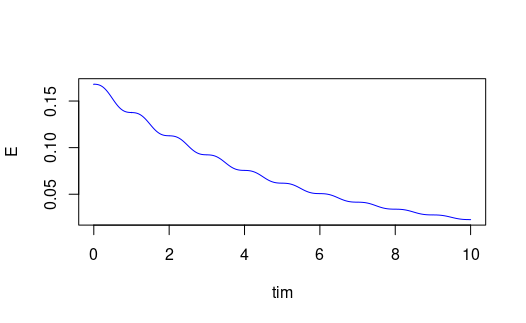
\includegraphics[width=0.5\textwidth]{gam02m1000.png}}
  \subfloat[$\gamma = 0$]{
    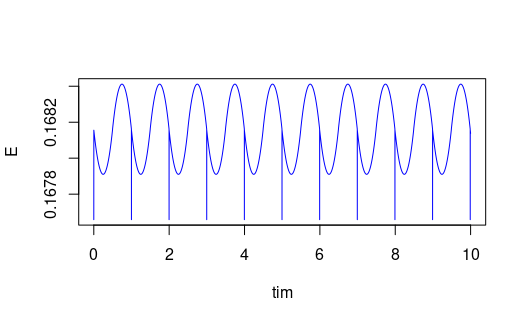
\includegraphics[width=0.5\textwidth]{gam0m1000.png}}
   \caption{Gràfics amb valor $M = 1000$}
\end{figure}
\hspace{-1.6em}\\S'observa com amb valor $M=1000$ obtenim el mateix comportament, però amb rangs de valors més petits; pel que la hipòtesis proposada ha estat corrovorada; les tendències cícliques de les gràfiques son degudes a problemes d'aproximació i, a mida que incrementem el valor del paràmetre $M$ (nombre d'intervals de la corda) aquesta discrepancia és menor i, aproximem millor l'energia de la corda, que a mida que augmenta el temps tendeix a 0 (en cas de $\gamma > 0$) o és manté constant (en cas de $\gamma = 0$).\\\\

\newpage
\section{Annex}\label{annex}
Exposem ara el codi programat per a obtenir les solucions dels sistemes proposats a l'entrega:
{\tiny
\begin{lstlisting}[language = GERONA]
u0 <- function(x) {x*(1-x)}
v0 = 0
c = 1
gam = 0.2
M <- 200
gt = 0
dx <- 1/(M)
mu <- 1
s <- 1
dt <- mu * dx ^ s
tfinal <- 10

Un = matrix(0, 1, M)
U0 = matrix(0, 1, M)
U_1 = matrix(0, 1, M)

A = matrix(0, M, M)
D = matrix(0, M, M)

for( m in 1:(M) ){
  U0[m] = u0(m*dx)
  U_1[m] = U0[m]
}
U_1 = t(U_1)
U0 = t(U0)

for( i in 1:(M) ){
  D[i, i] = 1+gam*dt
  
  A[i, i] = 2*(1-mu*mu)+gam*dt
  if( i > 1 ) { A[i, i-1] = mu*mu*c }
  if( i < M ) { A[i, i+1] = mu*mu*c }
}

D = solve(D)
RAZZ = function(Up, U) {
  RES = D%*%(A%*%U-Up)
  return(RES)
  }

Energy = function(Up, U){
  ret = c()
  for ( i in 2:(length(U)) ){
    res = ( ((U[i]-Up[i])/dt)**2+((U[i]-U[i-1])/dx)**2 )
    ret = c(ret, res)
  }
  ret = 0.5*sum(ret)* dx
  return(ret)
}

pos = c()
tim = c()

t = 0
E = c()

while (t <= tfinal) {
  Un = RAZZ(U_1, U0)
  
  Un[length(Un)] = 0
  Un[1] = 0
  
  En = Energy(U0, Un)
  
  pos = c(pos, Un[100])
  tim = c(tim,t)
  
  U_1 = U0
  U0 = Un
  
  E = c(E, En)
  
  t = t+dt
}

plot(tim, pos, col = 'purple', type ='l')
plot(tim, E, col = 'blue', type ='l')
\end{lstlisting}
}
\end{document}
